\chapter{Introduction}

\paragraph{\hspace{24pt}}
“A Cloud Computing model is a model which enables convenient, on demand network access to a shared pool of configurable computing resources and services. These resources include: networks, servers, storage, apps and services. These resources can be rapidly provisioned and released with minimal management effort or service provider interaction.”Cloud provides portability and flexibility of online services.

\paragraph{\hspace{24pt}}Introduction continues from 1.1 to 1.5. Chapter 2 of this paper discusses the key concerns of Data Security on Cloud. Chapter 3 discusses the various Issues. Chapter 4 discusses the Various Techniques to Secure Data on Cloud. Chapter 5 to 8 discuss about container clustering using docker and its working. Chapter 9 and 10 discuss about Kubernetes and why it is better than Docker Swarm.

\begin{figure}[htb]
\centering
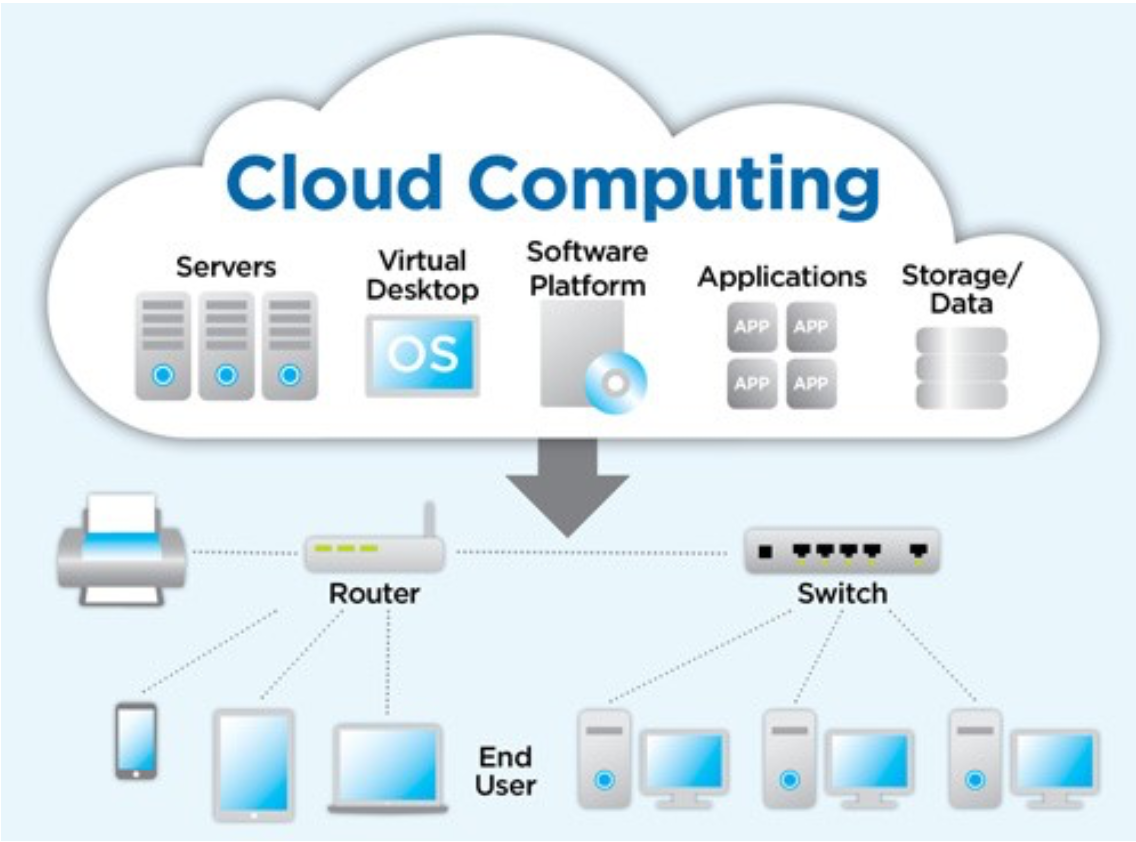
\includegraphics[width=10cm,height=6cm]{5-contents/1-Introduction/images/cloud-computing-intro.png} % e.g. insert ./image for image.png in the working directory, adjust scale as necessary
\caption{Cloud Computing}
\label{fig:label} % insert suitable label, this is used to refer to a fig from within the text as shown above
\end{figure}

\section{The Five Essential Characteristics}
\paragraph{\hspace{24pt}}
The Five essential characteristics of Cloud Computing are given below. These are vital features of this technology which define its usability and efficiency.\\
\textbf{1. On-Demand Self Service} {“A consumer can one-sidedly provision computing capabilities. These capabilities include server time and network storage. They can be provisioned whenever required without having human interaction with the service providers.”}\\
\textbf{2. Broad Network Access} {here are capabilities available over the network and can be accessed through various platforms such as mobile phones, laptops, PDAs and other electronic devices.}\\
\textbf{3. Resource Pooling} {The resources are amalgamated to serve multiple customers. This can be done with the help of multi-tenant models. These resources are dynamically assigned and reassigned depending on the consumer’s demands. Examples of such resources include storage, Memory, Processing, Network, Bandwidth and Virtual Machines.}\\
\textbf{4. Rapid Elasticity} {The capabilities can be provided elastically and rapidly, sometimes also automatically, for quick scale outs, and rapid releases to quickly scale in to the customer. Such capabilities are unlimited and can be bought whenever needed and in any quantity.}\\
\textbf{5. Measured Service} {The use of resources in cloud systems are automatically controlled and optimised. The usage of the services can be monitored and controlled. They can also be reported providing transparency for both, the provider and consumer.}

\section{The Three Service Models}
\paragraph{\hspace{24pt}}
There are three service models which are implanted in Cloud Computing. They are as follows:\\
\textbf{1. Infrastructure as a Service(IaaS)} {In IaaS, the consumer is provided with networks, storage, processing and various other computing resources. IaaS enables he consumer or user to deploy and execute the software. This software includes OSs and applications. The consumer is not in control of the cloud infrastructure. However, a consumer can control the OS, storage and the deployed apps. A consumer may also have partial control over selection of networking components such as host firewalls.}\\
\textbf{2. Platform as a Service (PaaS)} {PaaS allows the consumers to deploy their applications which are created using programming languages and various tools onto the cloud infrastructure. The control that the consumer has is similar to that of IaaS.}\\
\textbf{3. Software as a Service (SaaS)} {SaaS enables the consumer to use the capabilities such as applications which is provided by the service provider which runs on the infrastructure. These applications can be accessed from various devices through a thin client interface such as a web browser like Google Chrome, Mozilla Firefox, IE, Opera etc. The control that the consumer has is similar to that of IaaS and PaaS. However, the consumer may have partial control over user specific application configuration settings.}

\section{The Four Deployment Models}
\paragraph{\hspace{24pt}}
The cloud can be deployed in four different ways. They are as follows:\\

\begin{figure}[htb]
\centering
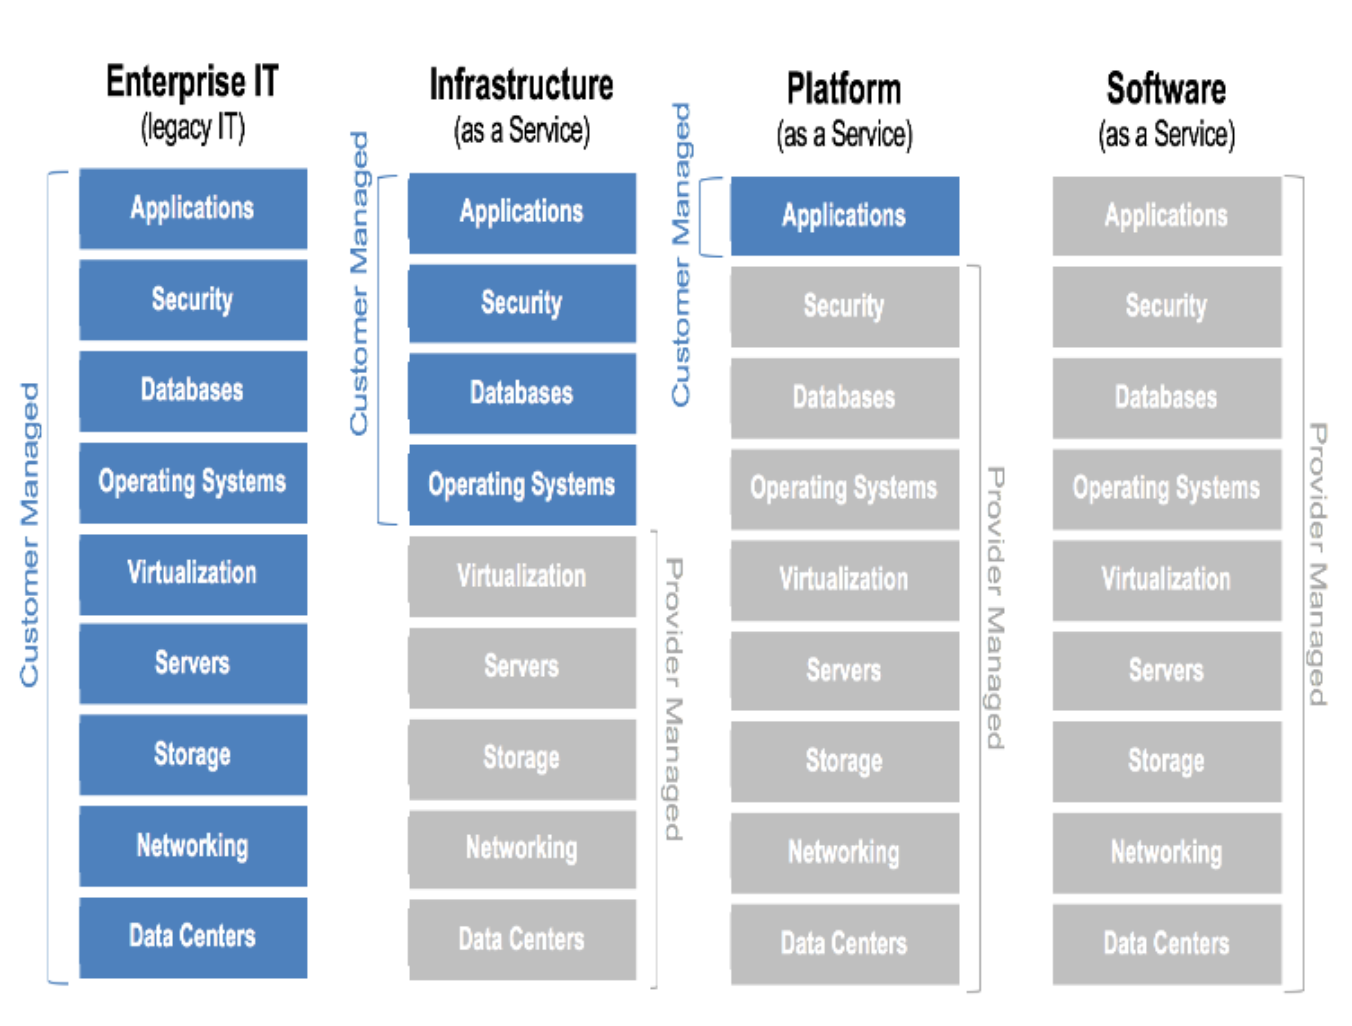
\includegraphics[width=12cm,height=8cm]{5-contents/1-Introduction/images/service-model.png} % e.g. insert ./image for image.png in the working directory, adjust scale as necessary
\caption{The Service Models}
\label{fig:label} % insert suitable label, this is used to refer to a fig from within the text as shown above
\end{figure}

\textbf{1. Public Cloud} {As the name suggests, this type of cloud is available to the general public. It is owned by organizations that sell cloud services. These service providers include Amazon’s Elastic Compute Cloud(EC2), Microsoft Azure Service Platform, Sun Cloud, Google App Engine, IBM’s Blue Cloud, etc.}\\
\textbf{2. Private Cloud} {This cloud infrastructure is operated solely for an organization. “The objective of a private cloud is not sell as-a-service offerings to external customers but to gain the benefits of cloud architecture without giving up the control of maintaining your own data centre.” A particular private cloud can be owned only by a single entity or organization.}\\
\textbf{3. Community Cloud} {The infrastructure of the community cloud is shared by multiple organizations. It supports a specific community that has similar or same concerns/issues. It may be managed by the organizations or a third party.}\\
\textbf{4. Hybrid Cloud} {A hybrid cloud is the incorporation of two or more clouds. Hybrid clouds can remain as unique entities. However, they are bound together by standardized technology that enables portability of data and applications.}
Users may use any of the deployment models as per their requirements and needs.

\begin{figure}[htb]
\centering
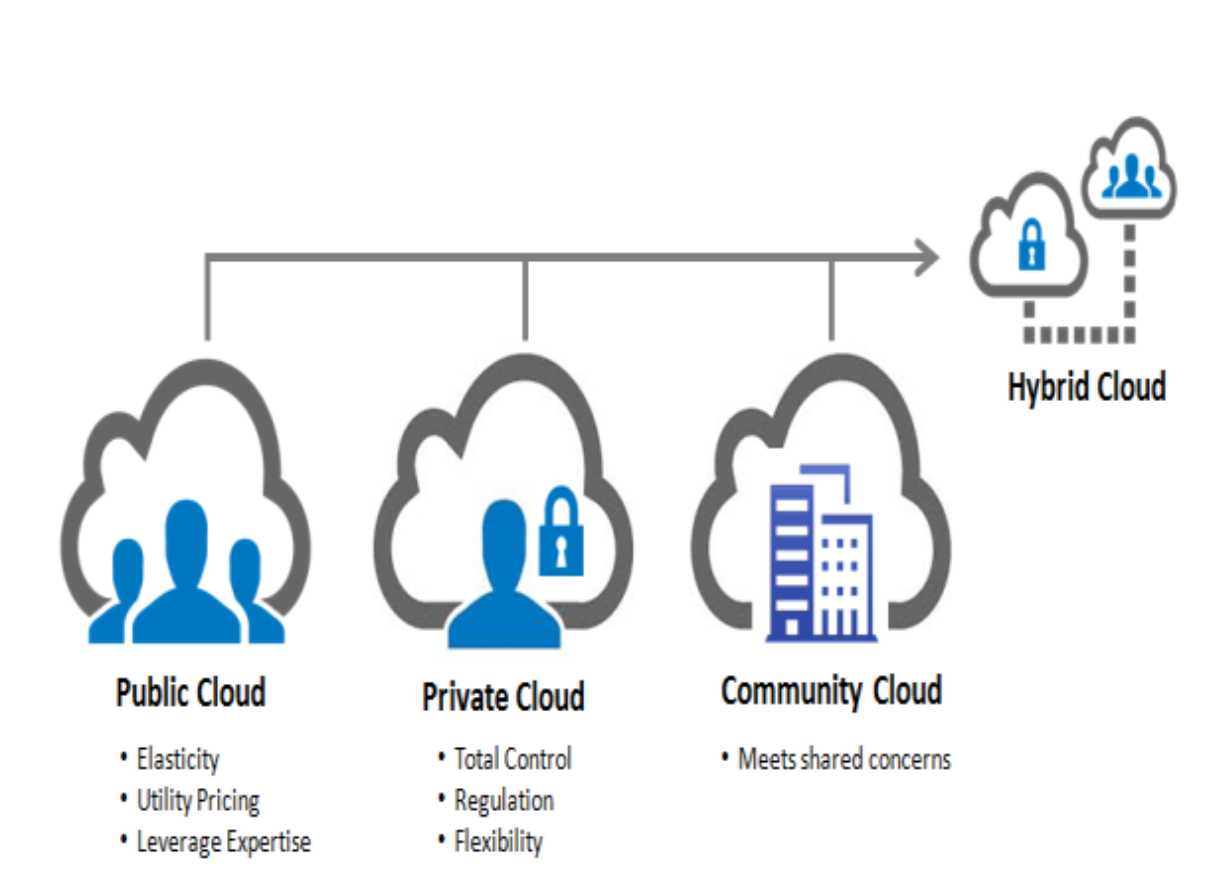
\includegraphics[width=12cm,height=8cm]{5-contents/1-Introduction/images/cloud-computing-model.png} % e.g. insert ./image for image.png in the working directory, adjust scale as necessary
\caption{Cloud Computing Models}
\label{fig:label} % insert suitable label, this is used to refer to a fig from within the text as shown above
\end{figure}

\section{Pros and Cons of Computing}
\paragraph{\hspace{24pt}}
Every technology has its own advantages and disadvantages. The pros and cons of Cloud Computing are as given below.

\subsection{Advantages}
\begin{enumerate}
    \item Minimized Costs
    \item Higher Resource Sharing.
    \item Consumption based cost.
    \item Efficient power saving.
    \item Faster time to deploy new services.
    \item Management moves to Cloud Provider
\end{enumerate}

\subsection{Disadvantages}
\begin{enumerate}
    \item Reliability
    \item Availability
    \item Security and Privacy Latency and Bandwidth guarantees.
    \item Absence of robust SLAs
    \item Uncertainty around inter-operablity, portability and lock-in.
    \item Compliance/Regulatory Laws mandate on-site ownership of data.
\end{enumerate}

\paragraph{\hspace{24pt}}
There are various advantages and disadvantages of Cloud Computing. Users must keep them in mind when they choose Cloud Computing for installing their applications or storing their data on Cloud servers.